\Chapter{COMMANDE OPTIMALE STOCHASTIQUE}\label{sec:Optimal_Control}
Ce chapitre est consacrée à l'étude du problème de commande optimale défini en (\ref{definition_optimal_control}).
\section{Formalisation du problème}
\paragraph{Dérivation de l'équation de programmation dynamique}\phantom{}\\
En reprenant la définition (\ref{value_function}) et en appliquant le principe d'optimalité de Bellman, il découle:
\begin{equation}\label{Bellman_optimality}
        F(x) = \inf_u\mathds{E}\left[\int_0^{\delta t}\left(\frac{1}{2}q\left[X_u(s)\right]u^2\left[X_u(s)\right]+r\left[X_u(s)\right]\right)ds+F(X_u(\delta t))\right]
\end{equation}
D'une part, pour $\delta t$ petit, il est possible d'écrire:
\begin{equation}\label{cost_function_simplification}
    \int_0^{\delta t}\left(\frac{1}{2}q\left[X_u(s)\right]u^2\left[X_u(s)\right]+r\left[X_u(s)\right]\right)ds=\left(\frac{1}{2}q(x){u(x)}^2+r(x)\right)\delta t+o(\delta t)
\end{equation}
D'autre part, un développement de Taylor combiné avec la formule d'Itô~\cite{ito1944} (appliquée au processus contrôlé de dynamique (\ref{controlled_process})) permet d'écrire (en supposant que $F\in C^2$):
\begin{equation}\label{taylor_ito}
    \begin{aligned}
        \mathds{E}[F(X_u(\delta t))]&=F(x)+\mathds{E}[dF(X_u(\delta t))]+o(\delta t)\\
        &=F(x)+\mathds{E}\left[F'(X_u(\delta t))dX_u(t)+\frac{1}{2}F''(X_u(\delta t))d{\langle X_u\rangle}_{\delta t} \right]+o(\delta t)\\
        &=F(x)+\left[a(b-x)+b(x)u(x)\right]F'(x)\delta t+\frac{1}{2}\sigma^2xF''(x)\delta t+o(\delta t)
    \end{aligned}
\end{equation}
où \({\langle X_u\rangle}_t\) dénote la variation quadratique du processus \(X_u(t)\).

En injectant (\ref{cost_function_simplification}) et (\ref{taylor_ito}) dans (\ref{Bellman_optimality}), il découle:
\begin{equation}\label{initial_minimisation problem}
    \begin{aligned}
        F(x)&=\inf_u\Bigg\{\left(\frac{1}{2}q(x){u(x)}^2+r(x)\right)\delta t+F(x)+\left[a(b-x)+b(x)u(x)\right]F'(x)\delta t\\&\quad\quad\quad\quad\quad\quad\quad\quad\quad\quad\quad\quad\quad\quad\quad\quad\quad\quad\quad\quad+\frac{1}{2}\sigma^2xF''(x)\delta t+o(\delta t)\Bigg\}
    \end{aligned}
\end{equation}
Ensuite, en retranchant $F(x)$ des deux côtés, en divisant partout par $\delta t$ et en prenant la limite lorsque $\delta t\to0$, l'équation de programmation dynamique est obtenue:
\begin{equation}\label{minimisation_problem}
    0=\min_u\left\{r(x)+\frac{1}{2}q(x)u^2(x)+[a(b-x)+b(x)u(x)]F'(x)+\frac{1}{2}\sigma^2xF''(x)\right\}
\end{equation}
\paragraph{Détermination de la commande optimale et dérivation de l'équation associée}\phantom{}\\
La minimisation à faire dans (\ref{minimisation_problem}) est en fonction de $u(x)$. Le terme à minimiser est:
\[
f(u(x))=\frac{1}{2}q(x){u(x)}^2+b(x)u(x)F'(x)
\]
La minimisation donne:
\begin{equation}\label{optimal_control}
    \begin{aligned}
        f'(u^*(x))&=0\\
        q(x)u^*(x)+b(x)F'(x)&=0\\
    u^*(x)&=-\frac{b(x)}{q(x)}F'(x)
    \end{aligned}
\end{equation}
Par ailleurs, la dérivée seconde est: 
\[
f''(u(x))=q(x)\quad\forall\;u(x)
\]
Puisque \( q(x) > 0 \) par hypothèse (\ref{definition_optimal_control}), la dérivée seconde par rapport au contrôle est strictement positive. L'expression de \( u^*(x) \) obtenue en (\ref{optimal_control}) réalise donc bien un minimum global. Il s'agit ainsi du contrôle optimal.

En injectant ce dernier (\ref{optimal_control}) dans (\ref{minimisation_problem}), l'équation \acl{HJB} est obtenue, régissant la fonction valeur associée à la commande optimale:
\begin{equation}\label{control_equation}
    r(x) - \frac{{b(x)}^2}{2q(x)}{\left[F'(x)\right]}^2 + a(b - x)F'(x) + \frac{1}{2}\sigma^2 x F''(x) = 0
\end{equation}
avec $F(0)=F(c)=0$ et $r(x)\neq0, b(x)\neq0, q(x)>0$.


\section{Résolution du problème sous différentes configurations}
\subsection{P1 \textemdash~Résolution}\label{p1}
\paragraph{Résolution du problème}\phantom{}\\
Il faut donc procéder à la résolution de l'équation (\ref{control_equation}). Whittle~\cite{whittle1982} a montré que la transformation: 
\[F(x)=-K\log(\varphi(x))\]
avec $\varphi(0)=\varphi(c)=1$ permet de linéariser l'équation en posant:
\[
K=\frac{\sigma^2xq(x)}{{b(x)}^2}
\]
L'équation devient:
\begin{equation}\label{linearised_equation}
    \frac{1}{2}\sigma^2 x\varphi''(x) + a(b - x)\varphi'(x) - \frac{r(x)}{K}\varphi(x) = 0
\end{equation}
Dans le cas où le terme suivant est constant:
\begin{equation}\label{condition}
    \frac{r(x)}{K}\equiv k\in\mathds{R}\;\forall\;x
\end{equation}
l'équation (\ref{linearised_equation}) est identique à celle de la \acl{FGM} $M(x;\alpha)$ pour:
\[
\alpha=\frac{r(x)}{K}
\]
Cela permet de résoudre une multitude de problèmes en supposant différentes formes pour $r(x)$, $b(x)$ et $q(x)$ tout en satisfaisant la condition (\ref{condition}). 

Soit les coûts suivants:
\begin{itemize}
    \item $r(x) = \rho$: coût immédiat constant, indépendant de l'état $x$ et du contrôle;
    \item $b(x) = \beta x$: coût du contrôle proportionnel à $x$ sur la dynamique;
    \item $q(x) = \kappa x$: poids pénalisant l'intensité du contrôle, linéaire avec $x$.
\end{itemize}

Cela donne:
\[
K=\frac{\kappa \sigma^2}{\beta^2}
\]
L'équation devient:
\begin{equation}\label{eq_exemple1}
    \frac{1}{2}\sigma^2 x\varphi''(x) + a(b - x)\varphi'(x) - \frac{\rho\beta^2}{\kappa \sigma^2}\varphi(x) = 0
\end{equation}
La solution est:
\[
\varphi(x)=C_1\Phi\left(\frac{\rho\beta^2}{a\kappa \sigma^2},\frac{2ab}{\sigma^2},\frac{2ax}{\sigma^2}\right) + C_2\Psi\left(\frac{\rho\beta^2}{a\kappa \sigma^2},\frac{2ab}{\sigma^2},\frac{2ax}{\sigma^2}\right)
\]
Les conditions aux limites $\varphi(0)=\varphi(1)=1$ permettent de déterminer les constantes $C_1$ et $C_2$:
\begin{equation}\label{control_constants}
    \begin{aligned}
        C_1=\frac{\Psi\left(\frac{\beta ^2 \rho }{a \kappa  \sigma ^2},\frac{2 a b}{\sigma ^2},0\right)-\Psi\left(\frac{\beta ^2 \rho }{a \kappa  \sigma ^2},\frac{2 a b}{\sigma ^2},\frac{2 a c}{\sigma ^2}\right)}{\Psi\left(\frac{\beta ^2 \rho }{a \kappa  \sigma ^2},\frac{2 a b}{\sigma ^2},0\right) \, \Phi\left(\frac{\beta ^2 \rho }{a \kappa  \sigma ^2};\frac{2 a b}{\sigma ^2};\frac{2 a c}{\sigma ^2}\right)-\Psi\left(\frac{\beta ^2 \rho }{a \kappa  \sigma ^2},\frac{2 a b}{\sigma ^2},\frac{2 a c}{\sigma ^2}\right)} \\
        C_2= \frac{\, \Phi\left(\frac{\beta ^2 \rho }{a \kappa  \sigma ^2};\frac{2 a b}{\sigma ^2};\frac{2 a c}{\sigma ^2}\right)-1}{\Psi\left(\frac{\beta ^2 \rho }{a \kappa  \sigma ^2},\frac{2 a b}{\sigma ^2},0\right) \, \Phi\left(\frac{\beta ^2 \rho }{a \kappa  \sigma ^2};\frac{2 a b}{\sigma ^2};\frac{2 a c}{\sigma ^2}\right)-\Psi\left(\frac{\beta ^2 \rho }{a \kappa  \sigma ^2},\frac{2 a b}{\sigma ^2},\frac{2 a c}{\sigma ^2}\right)}
    \end{aligned}
\end{equation}
L'expression analytique de la fonction valeur est donc:
\begin{equation}\label{sol_control_1}
    F(x)=-\frac{\kappa \sigma^2}{\beta^2} \log\left[C_1\Phi\left(\frac{\rho\beta^2}{a\kappa \sigma^2},\frac{2ab}{\sigma^2},\frac{2ax}{\sigma^2}\right) + C_2\Psi\left(\frac{\rho\beta^2}{a\kappa \sigma^2},\frac{2ab}{\sigma^2},\frac{2ax}{\sigma^2}\right)\right]
\end{equation}
Par ailleurs, le contrôle optimal est
\begin{equation}\label{optimal_control_1}
    u^*(x)=-\frac{\beta}{\kappa}F'(x)
\end{equation}

\subsection{P1 \textemdash~Visualisation}
La fonction valeur $F(x)$ (\ref{sol_control_1},~\ref{control_constants}) et le contrôle optimal (\ref{optimal_control_1}) sont tracés. D'abord, tous les paramètres des coûts sont fixés: $\rho=\beta=\kappa=1$.
\begin{figure}[htb]
    \centering
    \begin{subfigure}{0.45\linewidth}
        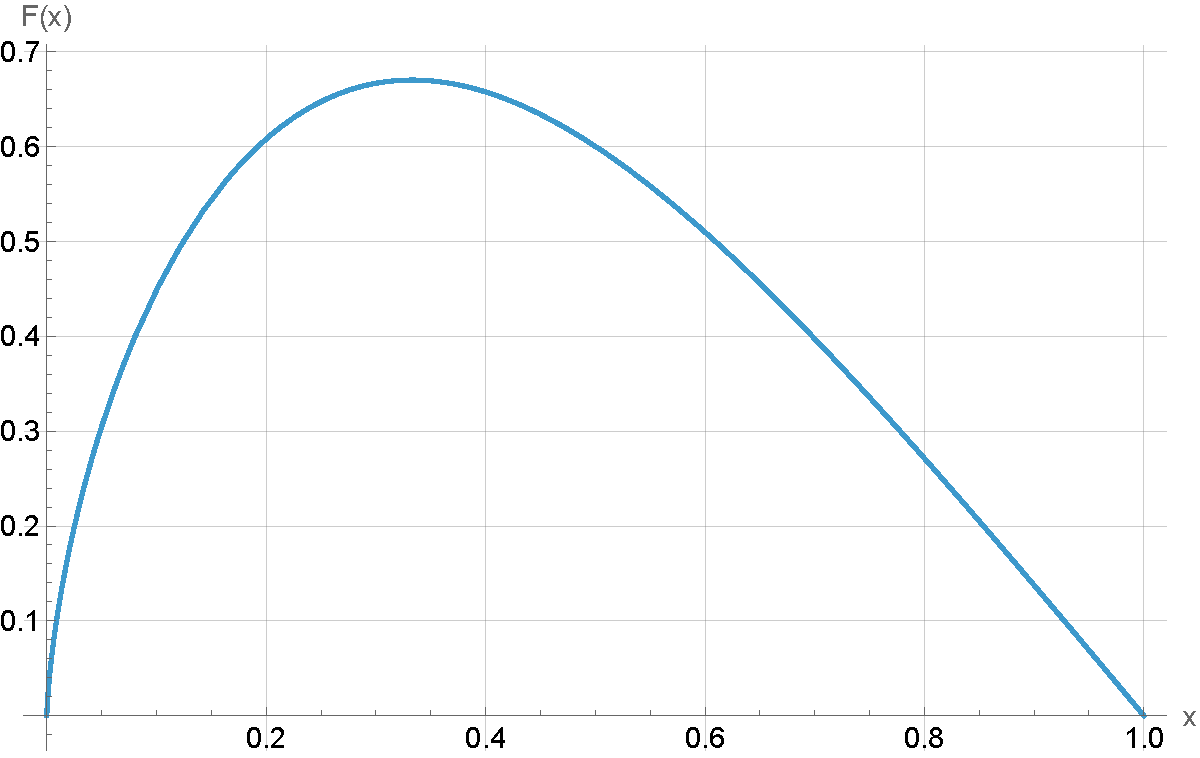
\includegraphics[width=\linewidth]{img/validation/P1/p1_value.pdf}
        \caption{P1 \textemdash~Fonction Valeur $F(x)$}\label{fig:ValueVisualisation1}
    \end{subfigure}
    \hfill
    \begin{subfigure}{0.45\linewidth}
        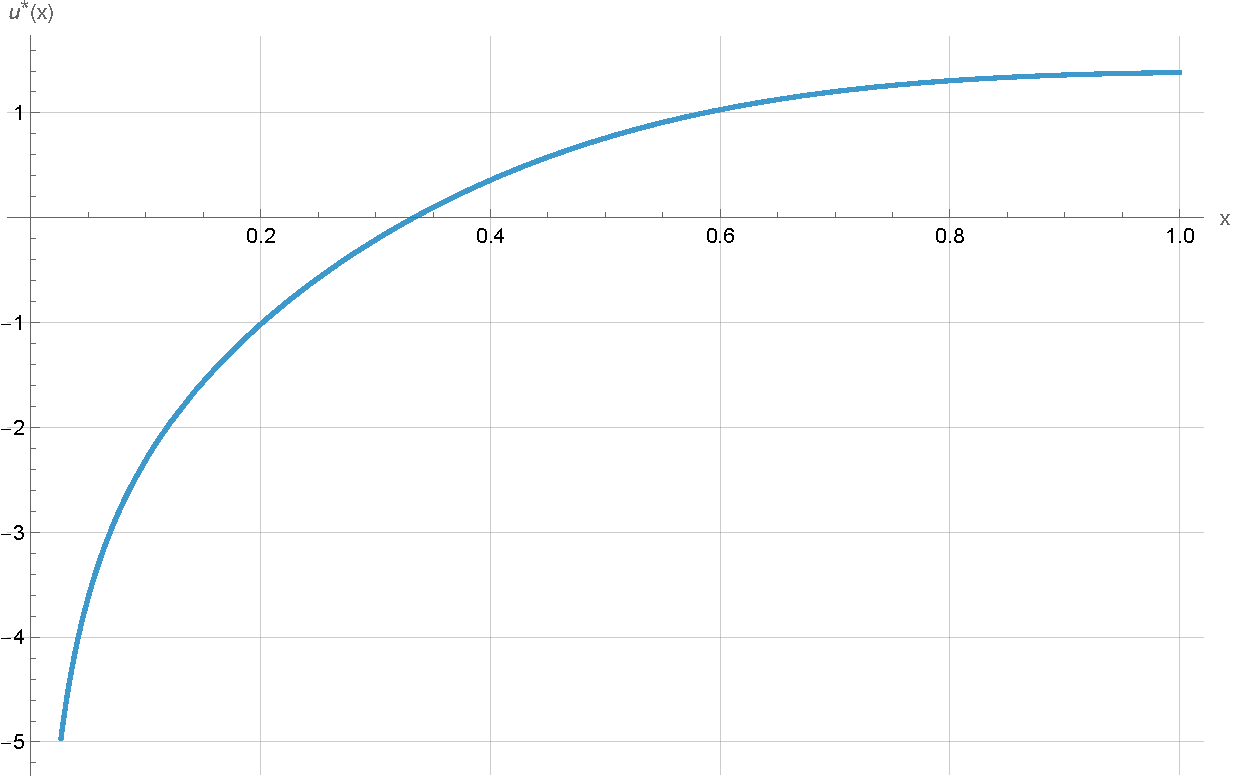
\includegraphics[width=\linewidth]{img/validation/P1/p1_control.pdf}
        \caption{P1 \textemdash~Contrôle Optimal $u^*(x)$}\label{fig:ControlVisualisation1}
    \end{subfigure}
    \caption{P1 \textemdash~Visualisation de la fonction valeur et du contrôle optimal}\label{fig:ValueControlComparison1}
\end{figure}\FloatBarrier De plus, il est intéressant d'analyser la sensibilité de ces fonctions par rapport à la variation des coûts. Les différentes valeurs des paramètres suivants sont évaluées:
\begin{itemize}
    \item Paramètre du coût immédiat $\rho,\;\forall\;\rho\in\{1,2,3,4\}$;
    \item Paramètre du coût de contrôle $\beta,\;\forall\;\beta\in\{1,2,3,4\}$;
    \item Paramètre du poids pénalisant l'intensité du contrôle $\kappa,\;\forall\;\kappa\in\{1,2,3,4\}$.
\end{itemize}
\begin{figure}[htb]
    \centering
    % Ligne 1 : Sensibilité à rho
    \begin{subfigure}{0.49\linewidth}
        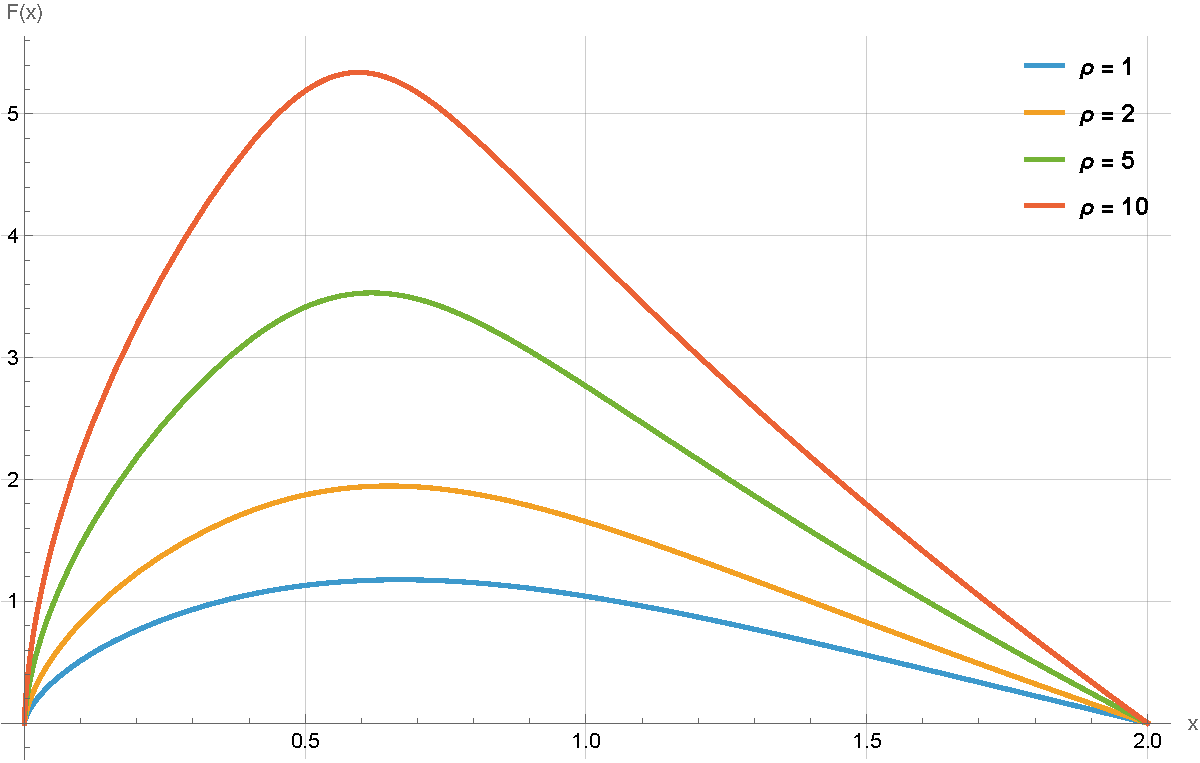
\includegraphics[width=\linewidth]{img/validation/P1/p1_R_value.pdf}
        \caption{P1 \textemdash~Fonction Valeur $F(x)$, $r(x)=\rho$}\label{fig:RhoValueVisualisation1}
    \end{subfigure}
    \hfill
    \begin{subfigure}{0.49\linewidth}
        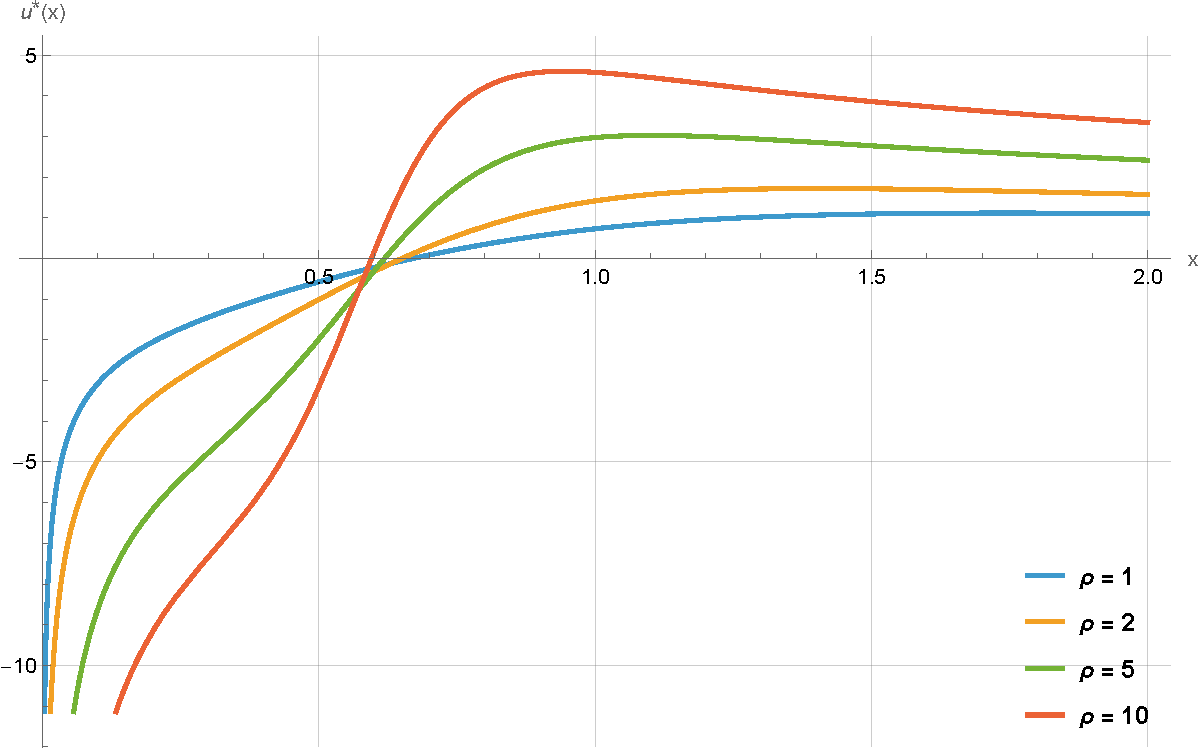
\includegraphics[width=\linewidth]{img/validation/P1/p1_R_control.pdf}
        \caption{P1 \textemdash~Contrôle Optimal $u^*(x)$, $r(x)=\rho$}\label{fig:RhoControlVisualisation1}
    \end{subfigure}

    % Ligne 2 : Sensibilité à beta
    \begin{subfigure}{0.49\linewidth}
        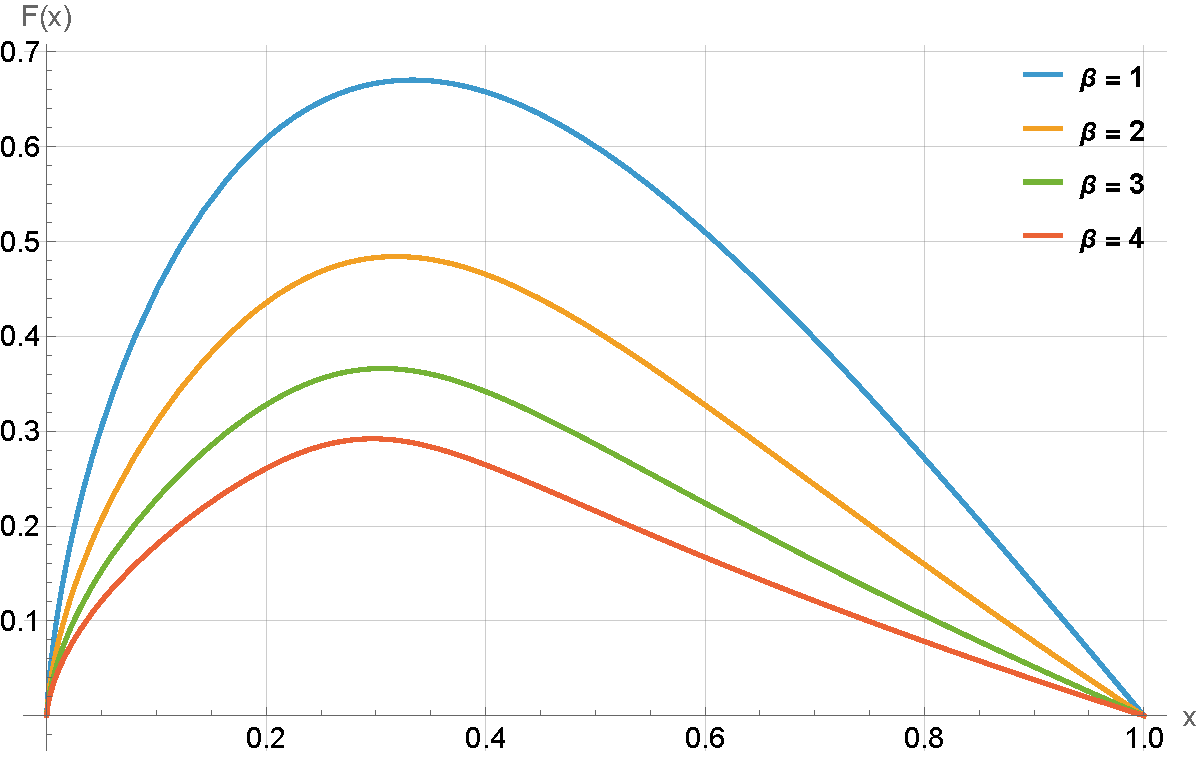
\includegraphics[width=\linewidth]{img/validation/P1/p1_B_value.pdf}
        \caption{P1 \textemdash~Fonction Valeur $F(x)$, $b(x)=\beta x$}\label{fig:BetaValueVisualisation1}
    \end{subfigure}
    \hfill
    \begin{subfigure}{0.49\linewidth}
        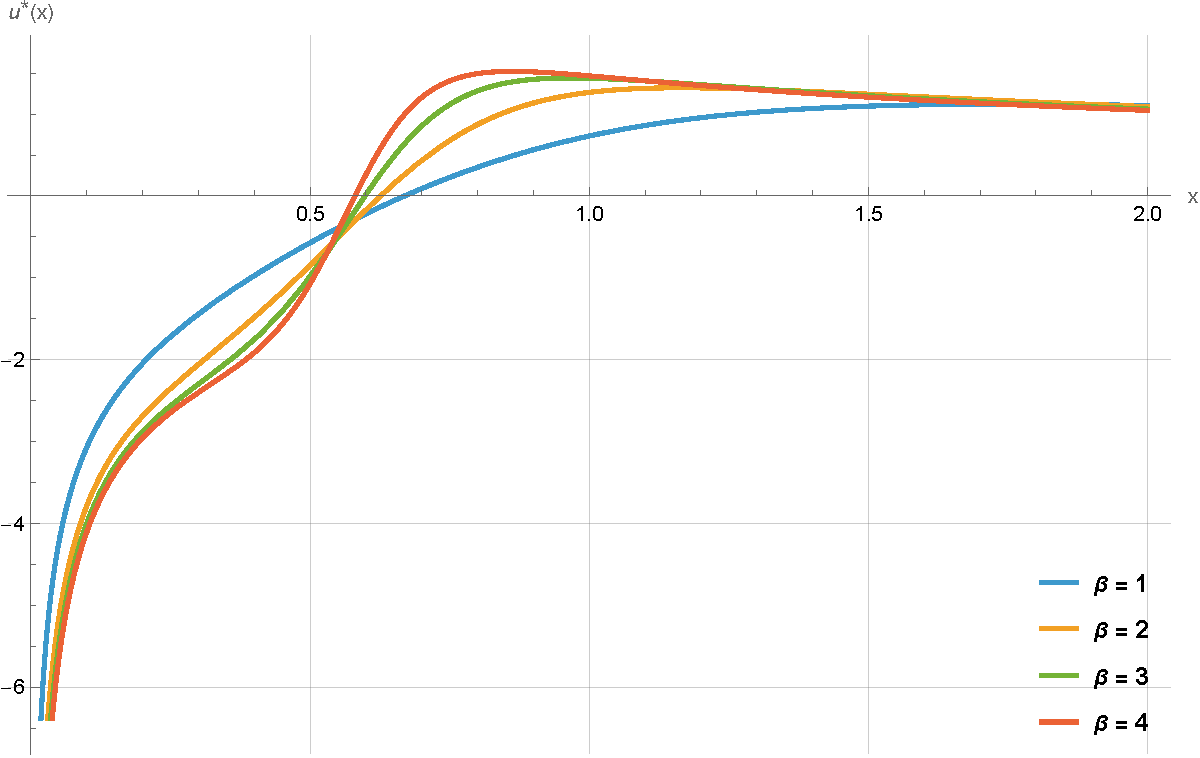
\includegraphics[width=\linewidth]{img/validation/P1/p1_B_control.pdf}
        \caption{P1 \textemdash~Contrôle Optimal $u^*(x)$, $b(x)=\beta x$}\label{fig:BetaControlVisualisation1}
    \end{subfigure}

    % Ligne 3 : Sensibilité à kappa
    \begin{subfigure}{0.49\linewidth}
        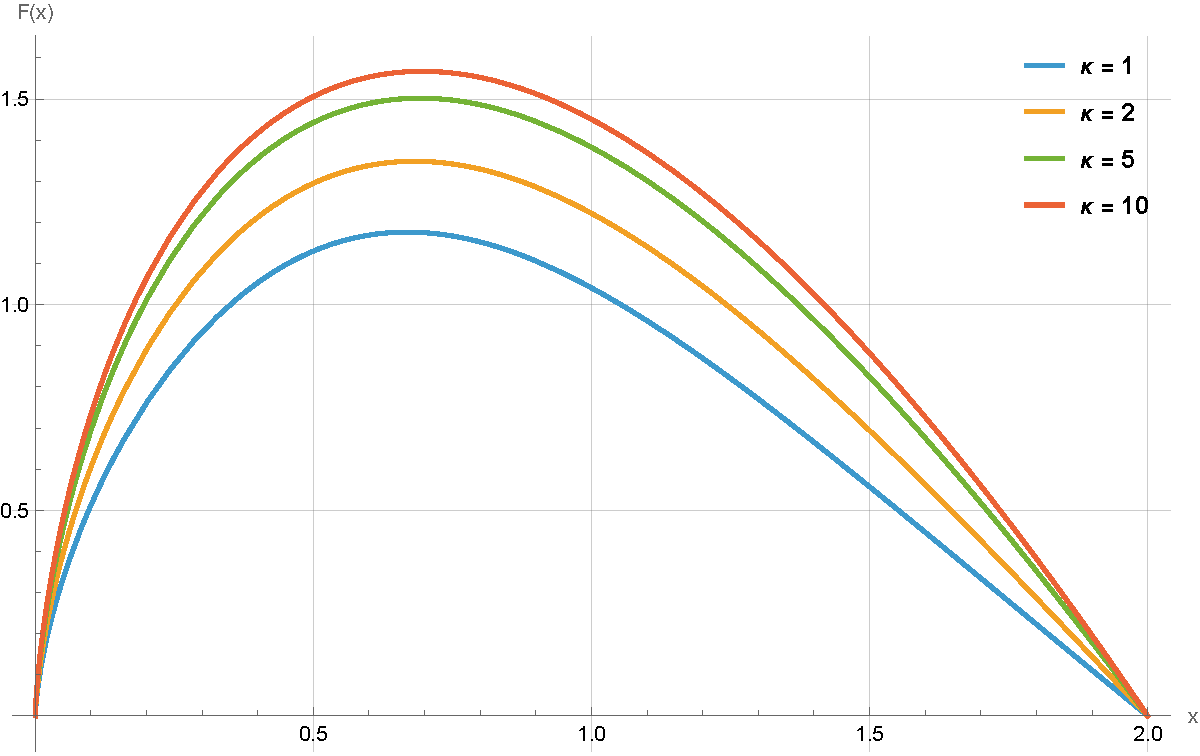
\includegraphics[width=\linewidth]{img/validation/P1/p1_K_value.pdf}
        \caption{P1 \textemdash~Fonction Valeur $F(x)$, $q(x)=\kappa x$}\label{fig:KappaValueVisualisation1}
    \end{subfigure}
    \hfill
    \begin{subfigure}{0.49\linewidth}
        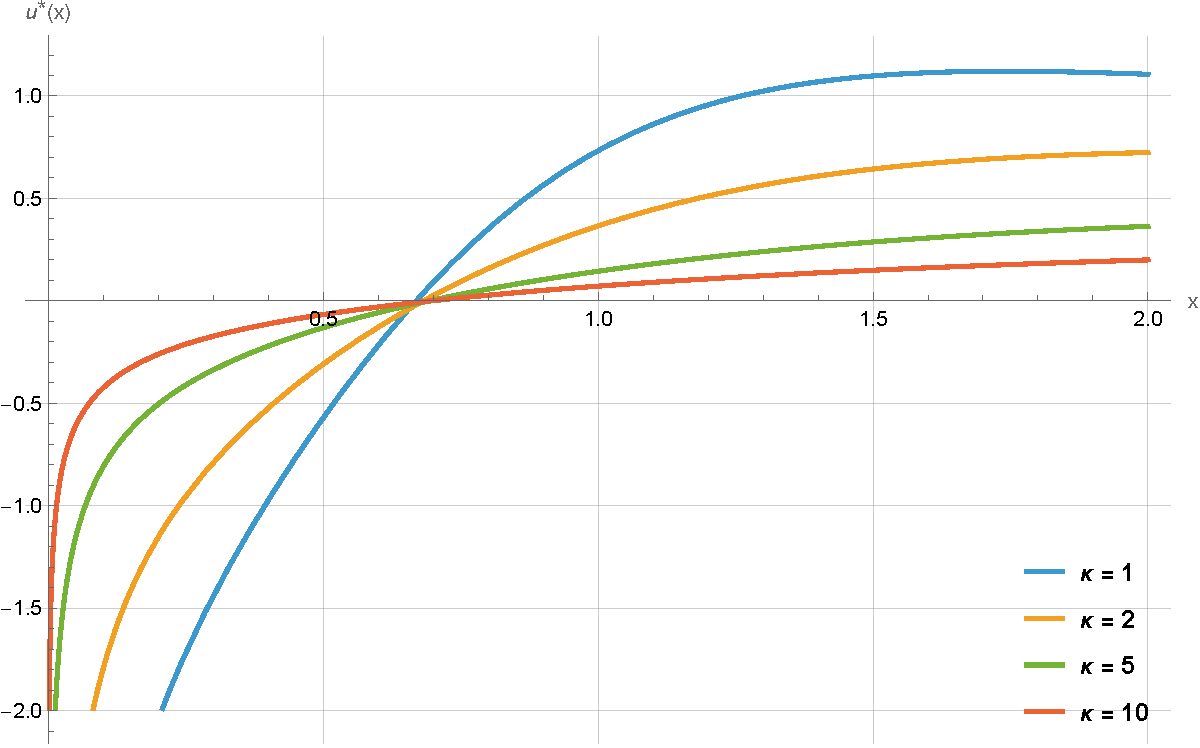
\includegraphics[width=\linewidth]{img/validation/P1/p1_K_control.pdf}
        \caption{P1 \textemdash~Contrôle Optimal $u^*(x)$, $q(x)=\kappa x$}\label{fig:KappaControlVisualisation1}
    \end{subfigure}

    \caption{P1 \textemdash~Sensibilité des fonctions valeur $F(x)$ et contrôle optimal $u^*(x)$}
    \label{fig:ParamSensitivityP1}
\end{figure}
\FloatBarrier Par ailleurs, une simulation d'une trajectoire contrôlée et d'une trajectoire non contrôlée est effectuée en utilisant un même tirage aléatoire, afin de permettre une comparaison pertinente entre les deux dynamiques.
\begin{figure}[htb]
    \centering
    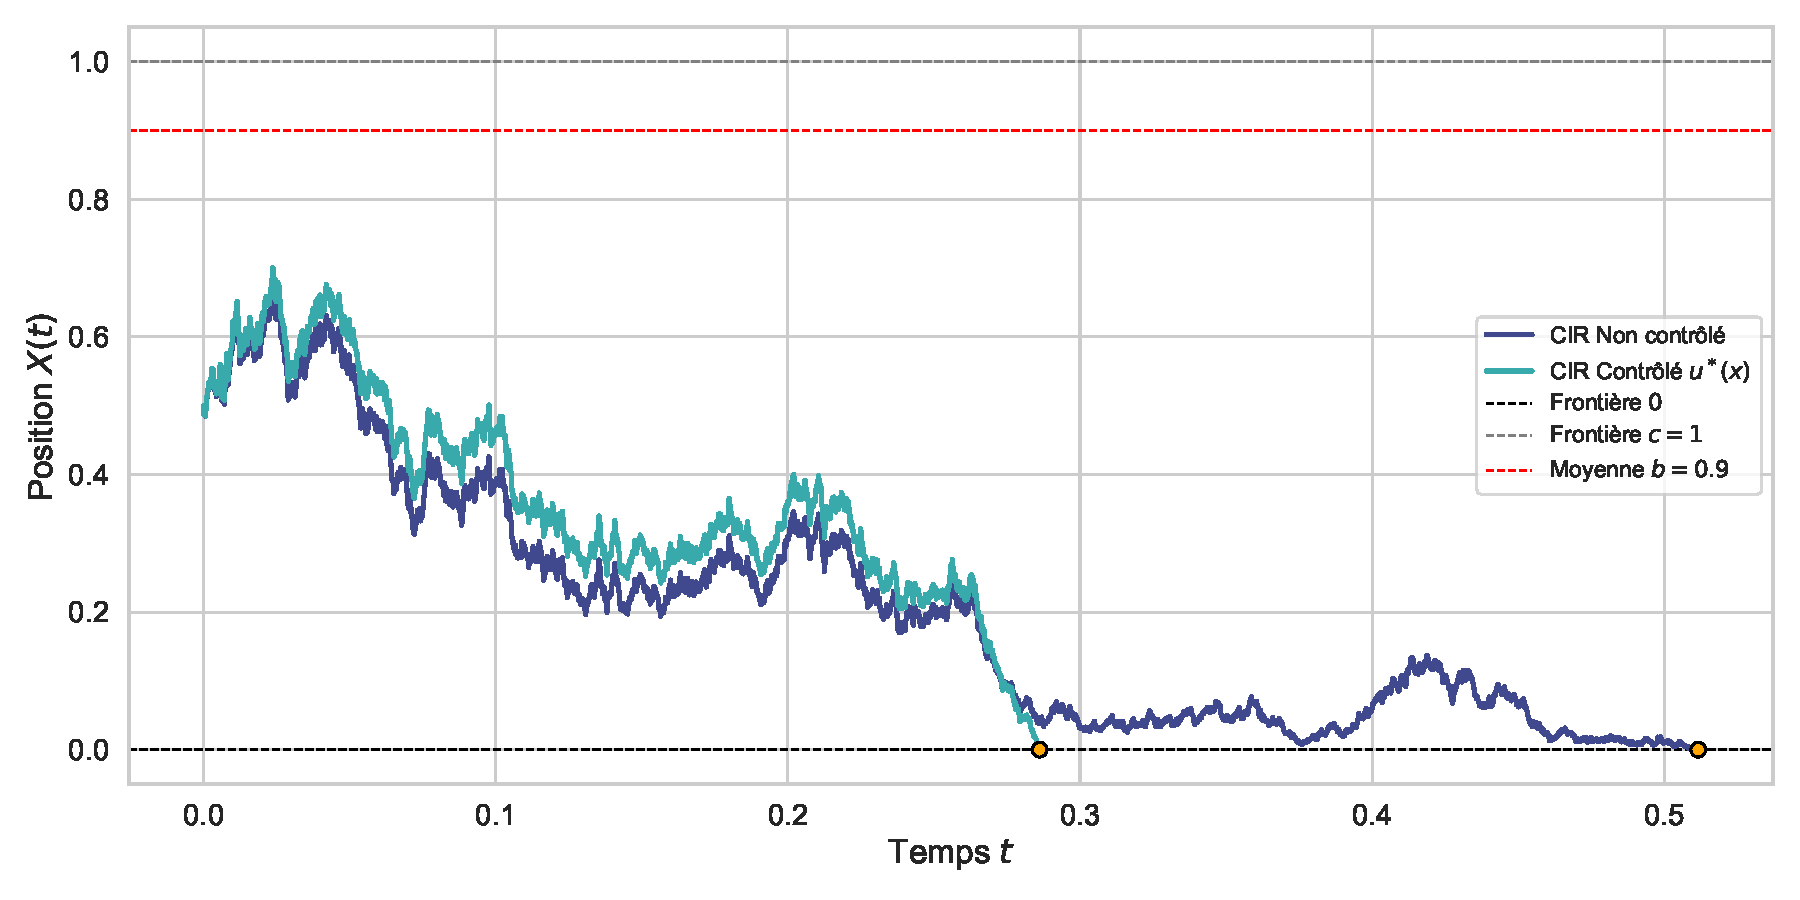
\includegraphics[width=0.9\linewidth]{img/validation/P1/p1_control_simulation.pdf}
    \caption{P1 \textemdash~Visualisation de l'effet de la commande optimale}\label{fig:Simulation1}
\end{figure}\FloatBarrier\subsection{P2 \textemdash~Résolution}\label{p2}
\noindent Soit le problème suivant: 
\begin{itemize}
    \item $r(x) = \rho x$: coût immédiat linéaire en $x$, indépendant du contrôle;
    \item $b(x) = \beta \sqrt{x}$: coût du contrôle proportionnel à $\sqrt{x}$;
    \item $q(x) = \kappa x$: poids pénalisant l'intensité du contrôle, linéaire avec $x$.
\end{itemize}
De la même manière que pour P1, il est possible de linéariser en posant: 
\[
K=\frac{x\kappa \sigma^2}{\beta^2}
\]
L'équation obtenue est identique à celle du premier problème (\ref{eq_exemple1}): 
\[
\frac{1}{2}\sigma^2 x\varphi''(x) + a(b - x)\varphi'(x) - \frac{\rho\beta^2}{\kappa \sigma^2}\varphi(x) = 0
\]
L'expression de $\varphi(x)$ est donc la même. Il en découle alors l'expression de la solution $F(x)$: 
\begin{equation}\label{sol_control_2}
    F(x)=-\frac{x\kappa \sigma^2}{\beta^2}\log\left[C_1\Phi\left(\frac{\rho\beta^2}{a\kappa \sigma^2},\frac{2ab}{\sigma^2},\frac{2ax}{\sigma^2}\right) + C_2\Psi\left(\frac{\rho\beta^2}{a\kappa \sigma^2},\frac{2ab}{\sigma^2},\frac{2ax}{\sigma^2}\right)\right]
\end{equation}

Par ailleurs, le contrôle optimal est
\begin{equation}\label{optimal_control_2}
    u^*(x)=-\frac{\beta}{\kappa\sqrt{x}}F'(x)
\end{equation}
\subsection{P2 \textemdash~Visualisation}
La fonction valeur $F(x)$ (\ref{sol_control_2},~\ref{control_constants}) et le contrôle optimal (\ref{optimal_control_1}) sont tracés. Dans un premier temps, tous les paramètres des coûts sont: $\rho=\beta=\kappa=1$.
\begin{figure}[htb]
    \centering
    \begin{subfigure}{0.45\linewidth}
        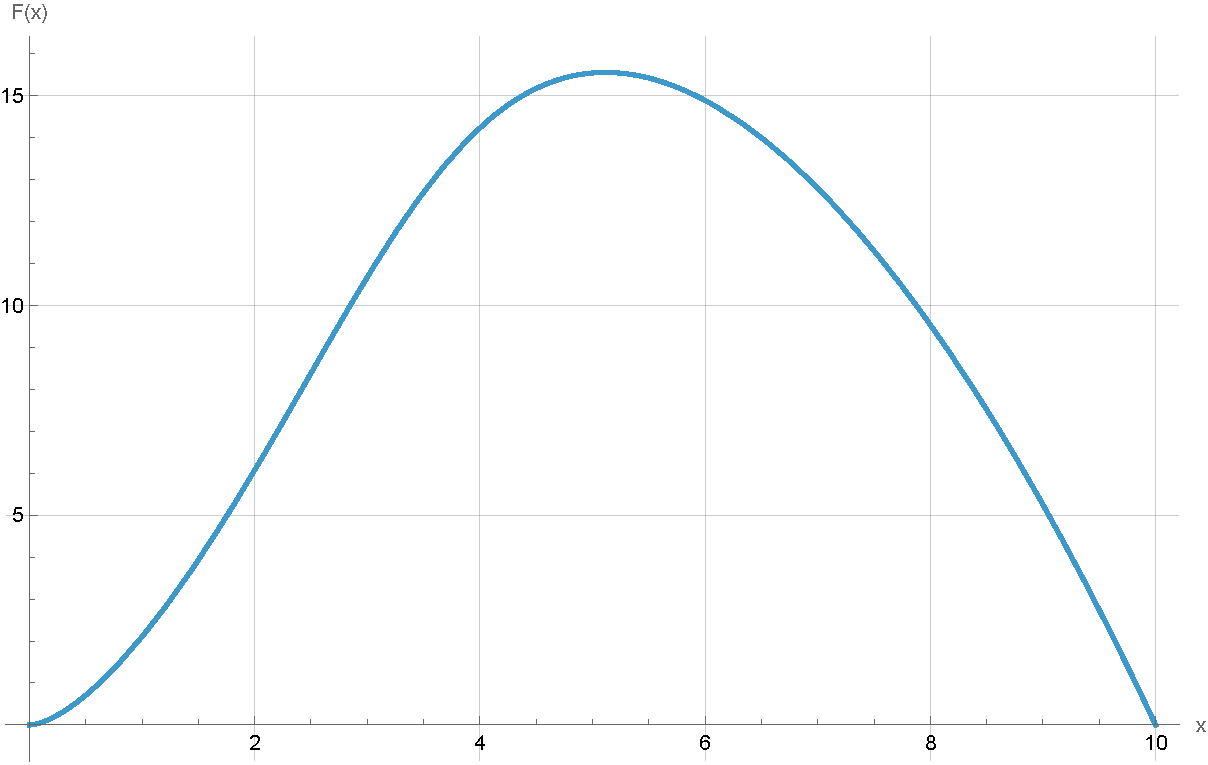
\includegraphics[width=\linewidth]{img/validation/P2/p2_value.pdf}
        \caption{P2 \textemdash~Fonction Valeur $F(x)$}\label{fig:ValueVisualisation2}
    \end{subfigure}
    \hfill
    \begin{subfigure}{0.45\linewidth}
        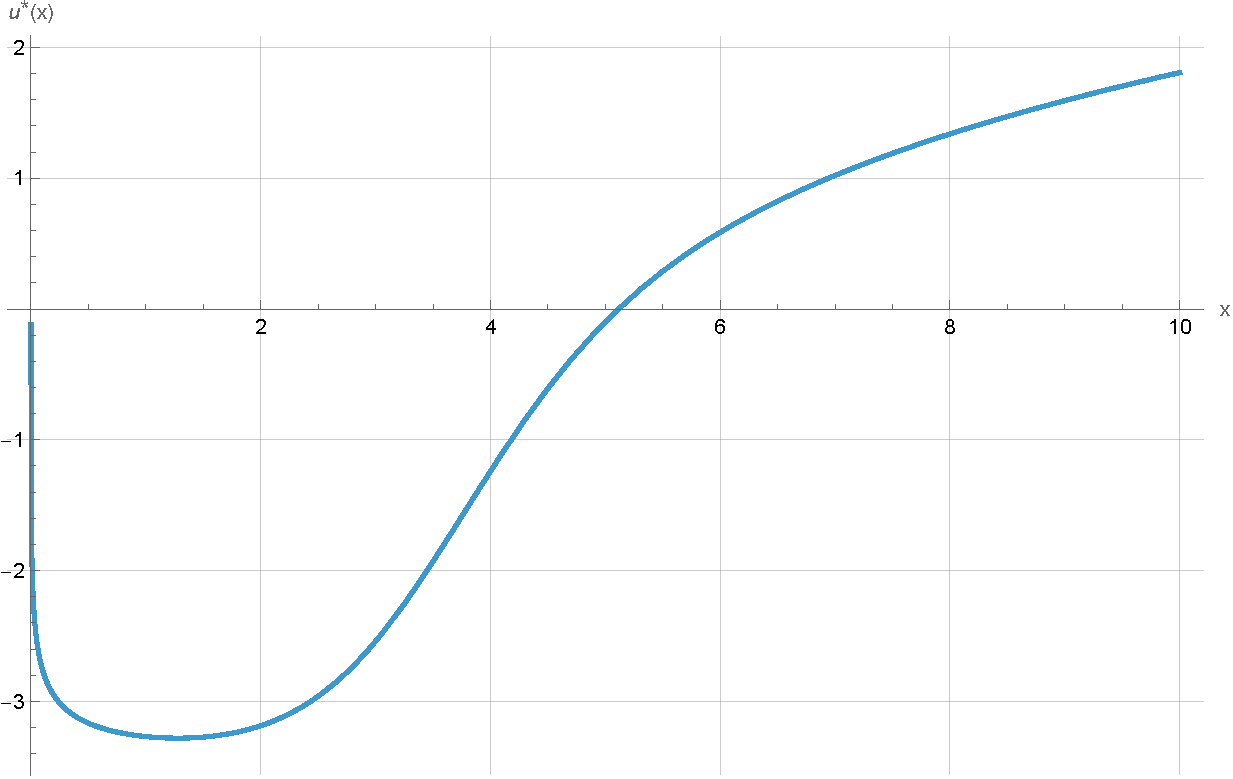
\includegraphics[width=\linewidth]{img/validation/P2/p2_control.pdf}
        \caption{P2 \textemdash~Contrôle Optimal $u^*(x)$}\label{fig:ControlVisualisation2}
    \end{subfigure}
    \caption{P2 \textemdash~Visualisation de la fonction valeur et du contrôle optimal}\label{fig:ValueControlComparison2}
\end{figure}\FloatBarrier Dans un second temps, et comme ce qui précède, la sensibilité des coûts est analysée, en fonction des mêmes valeurs paramètres $\rho$, $\beta$ et $\kappa$.
\begin{figure}[htb]
    \centering
    % Ligne 1 : Sensibilité à rho
    \begin{subfigure}{0.45\linewidth}
        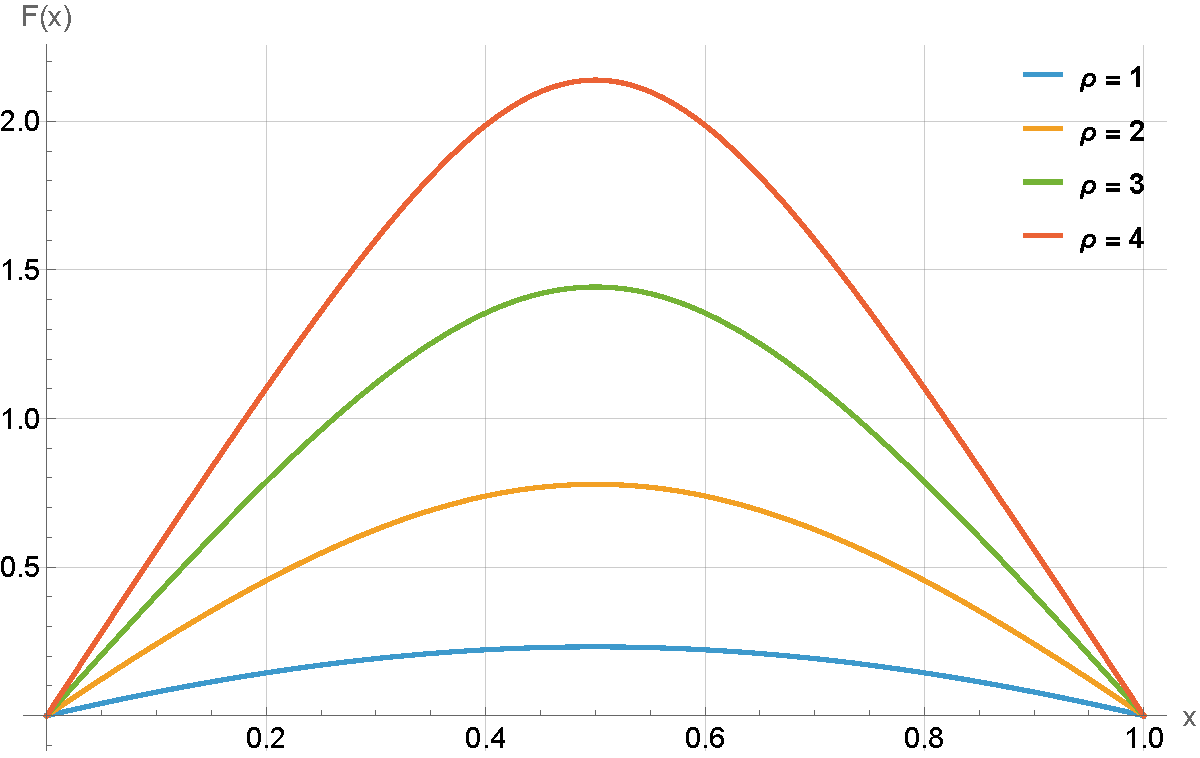
\includegraphics[width=\linewidth]{img/validation/P2/p2_R_value.pdf}
        \caption{P2 \textemdash~Fonction Valeur $F(x)$, $r(x)=\rho x$}\label{fig:RhoValueVisualisation2}
    \end{subfigure}
    \hfill
    \begin{subfigure}{0.45\linewidth}
        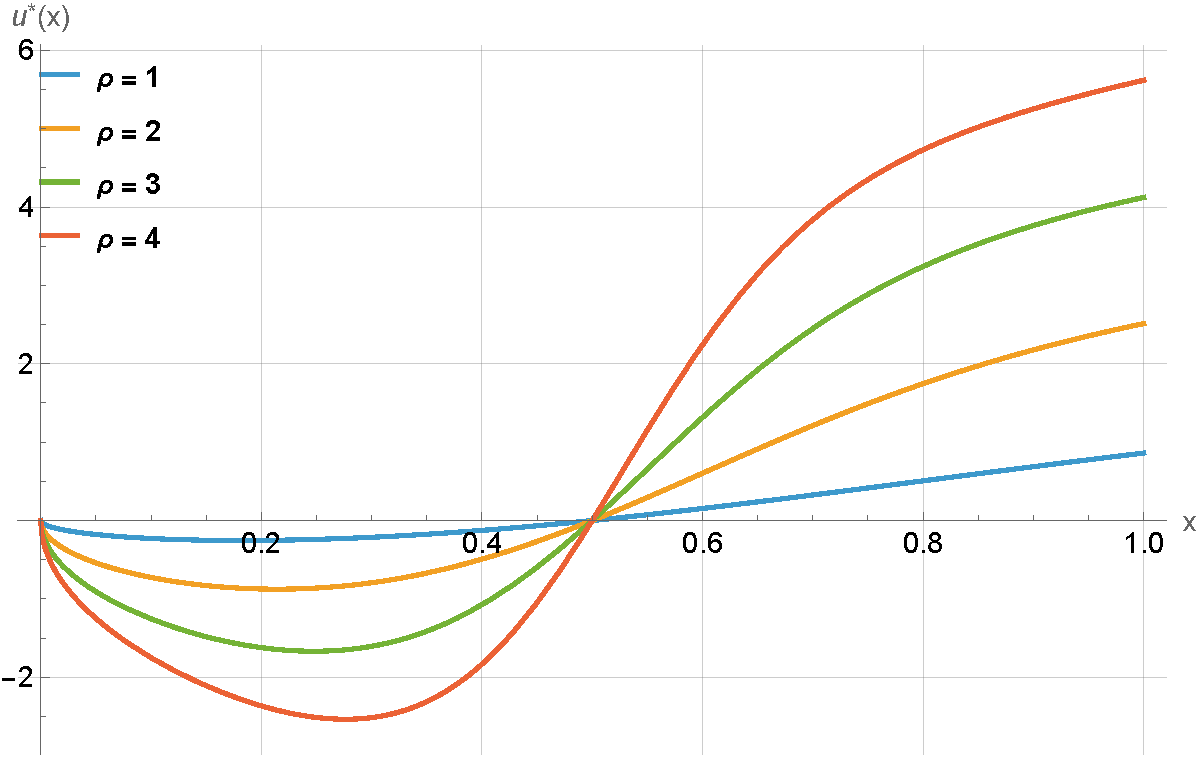
\includegraphics[width=\linewidth]{img/validation/P2/p2_R_control.pdf}
        \caption{P2 \textemdash~Contrôle Optimal $u^*(x)$, $r(x)=\rho x$}\label{fig:RhoControlVisualisation2}
    \end{subfigure}

    % Ligne 2 : Sensibilité à beta
    \begin{subfigure}{0.45\linewidth}
        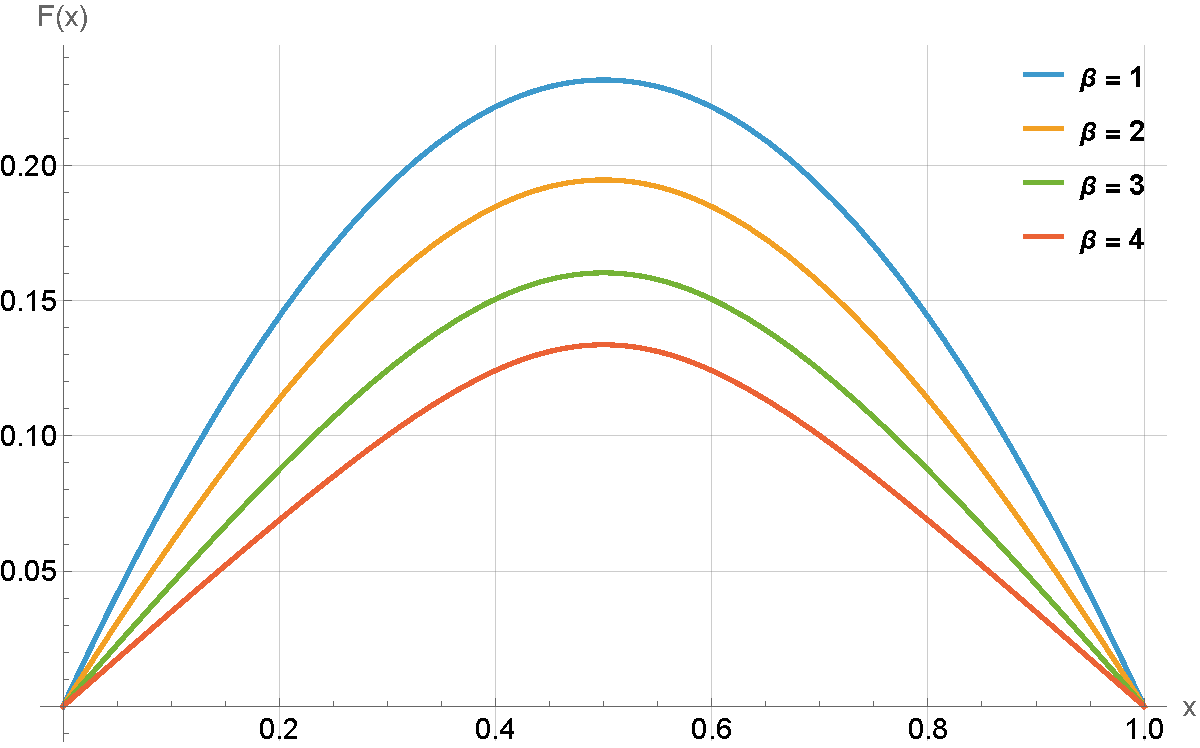
\includegraphics[width=\linewidth]{img/validation/P2/p2_B_value.pdf}
        \caption{P2 \textemdash~Fonction Valeur $F(x)$, $b(x)=\beta \sqrt{x}$}\label{fig:BetaValueVisualisation2}
    \end{subfigure}
    \hfill
    \begin{subfigure}{0.45\linewidth}
        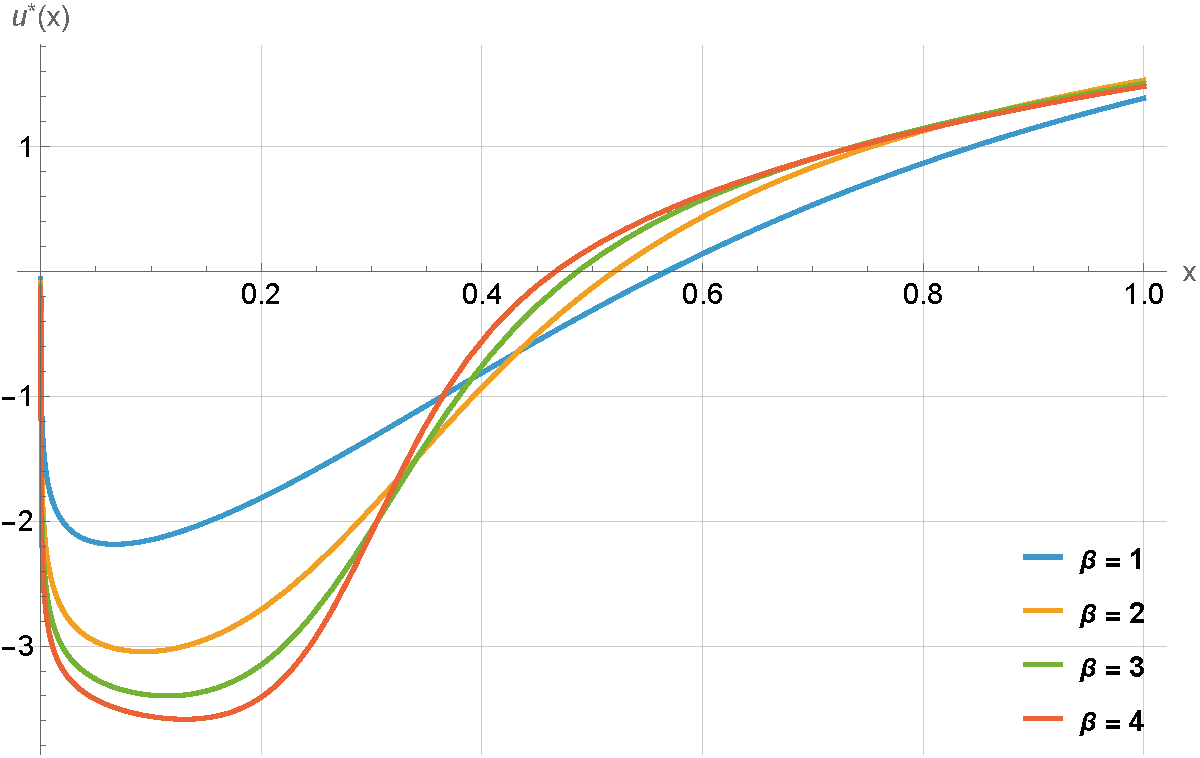
\includegraphics[width=\linewidth]{img/validation/P2/p2_B_control.pdf}
        \caption{P2 \textemdash~Contrôle Optimal $u^*(x)$, $b(x)=\beta \sqrt{x}$}\label{fig:BetaControlVisualisation2}
    \end{subfigure}

    % Ligne 3 : Sensibilité à kappa
    \begin{subfigure}{0.45\linewidth}
        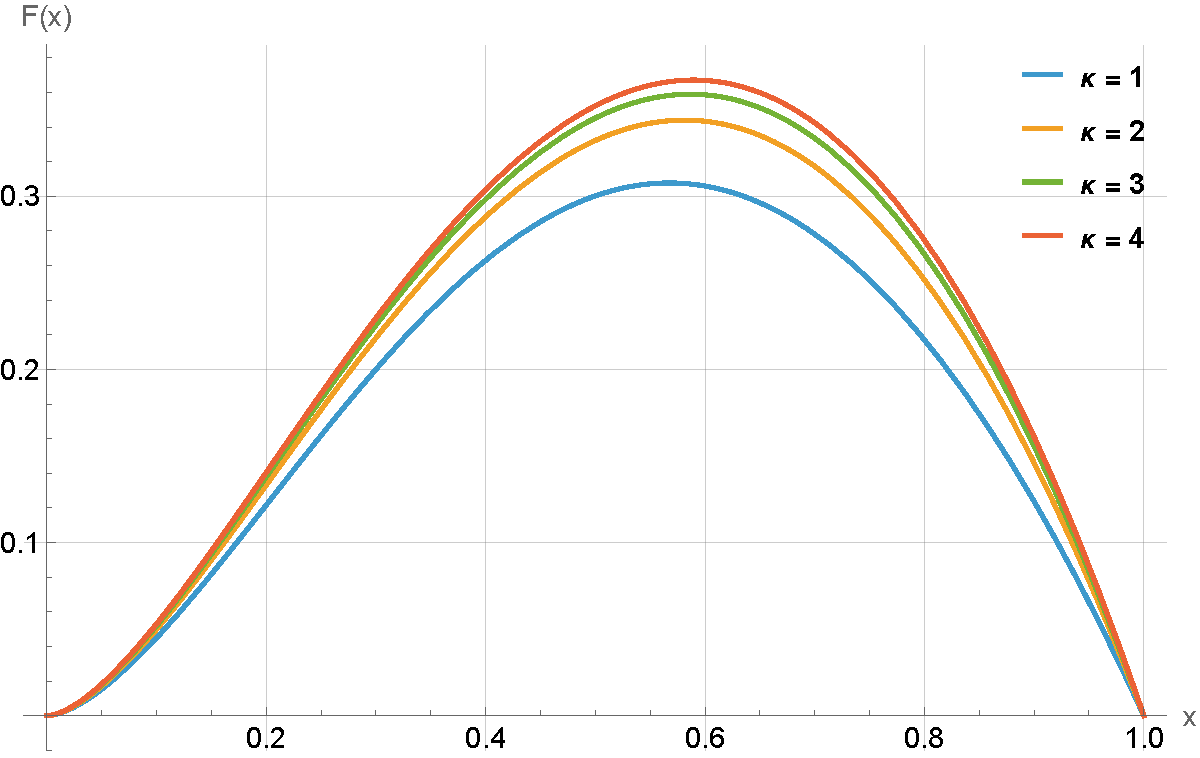
\includegraphics[width=\linewidth]{img/validation/P2/p2_K_value.pdf}
        \caption{P2 \textemdash~Fonction Valeur $F(x)$, $q(x)=\kappa x$}\label{fig:KappaValueVisualisation2}
    \end{subfigure}
    \hfill
    \begin{subfigure}{0.45\linewidth}
        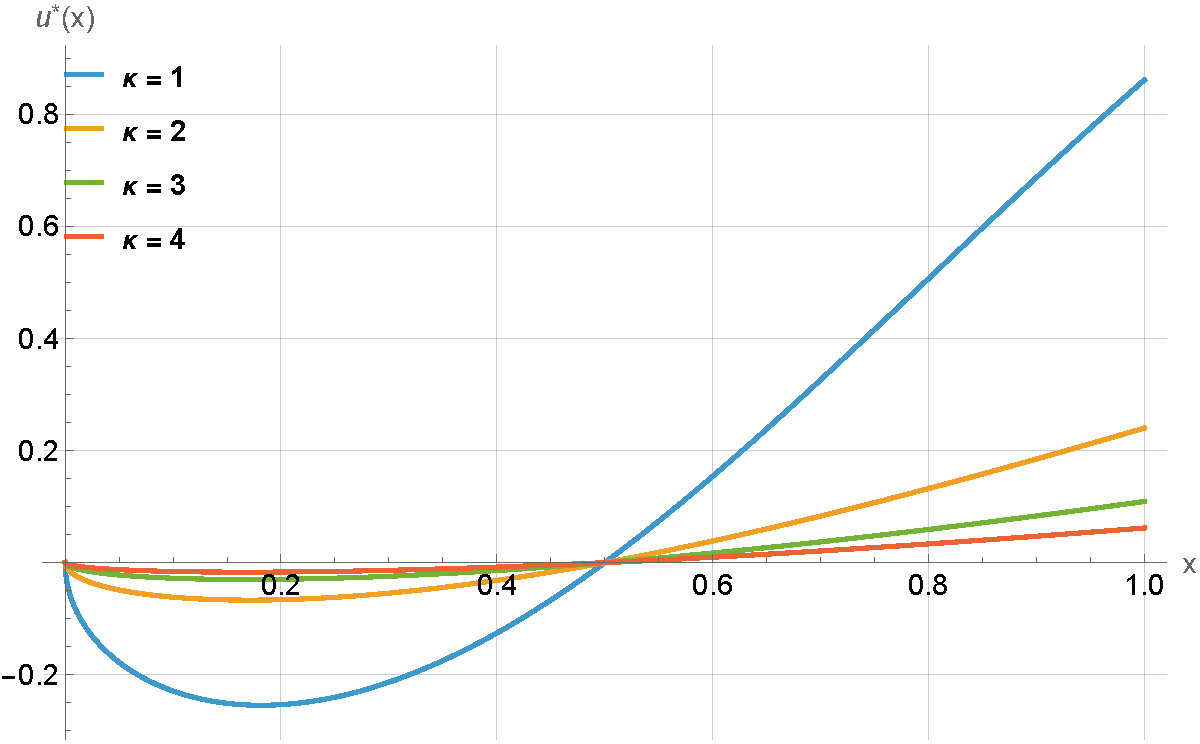
\includegraphics[width=\linewidth]{img/validation/P2/p2_K_control.pdf}
        \caption{P2 \textemdash~Contrôle Optimal $u^*(x)$, $q(x)=\kappa x$}\label{fig:KappaControlVisualisation2}
    \end{subfigure}

    \caption{P2 \textemdash~Sensibilité des fonctions valeur $F(x)$ et contrôle optimal $u^*(x)$}\label{fig:ParamSensitivityP2}
\end{figure}
\FloatBarrier Enfin, et comme précédemment, une trajectoire contrôlée est comparée à une trajectoire non contrôlée à partir d'un même tirage aléatoire. Les paramètres utilisés sont identiques à ceux de la dernière simulation.
\begin{figure}[htb]
    \centering
    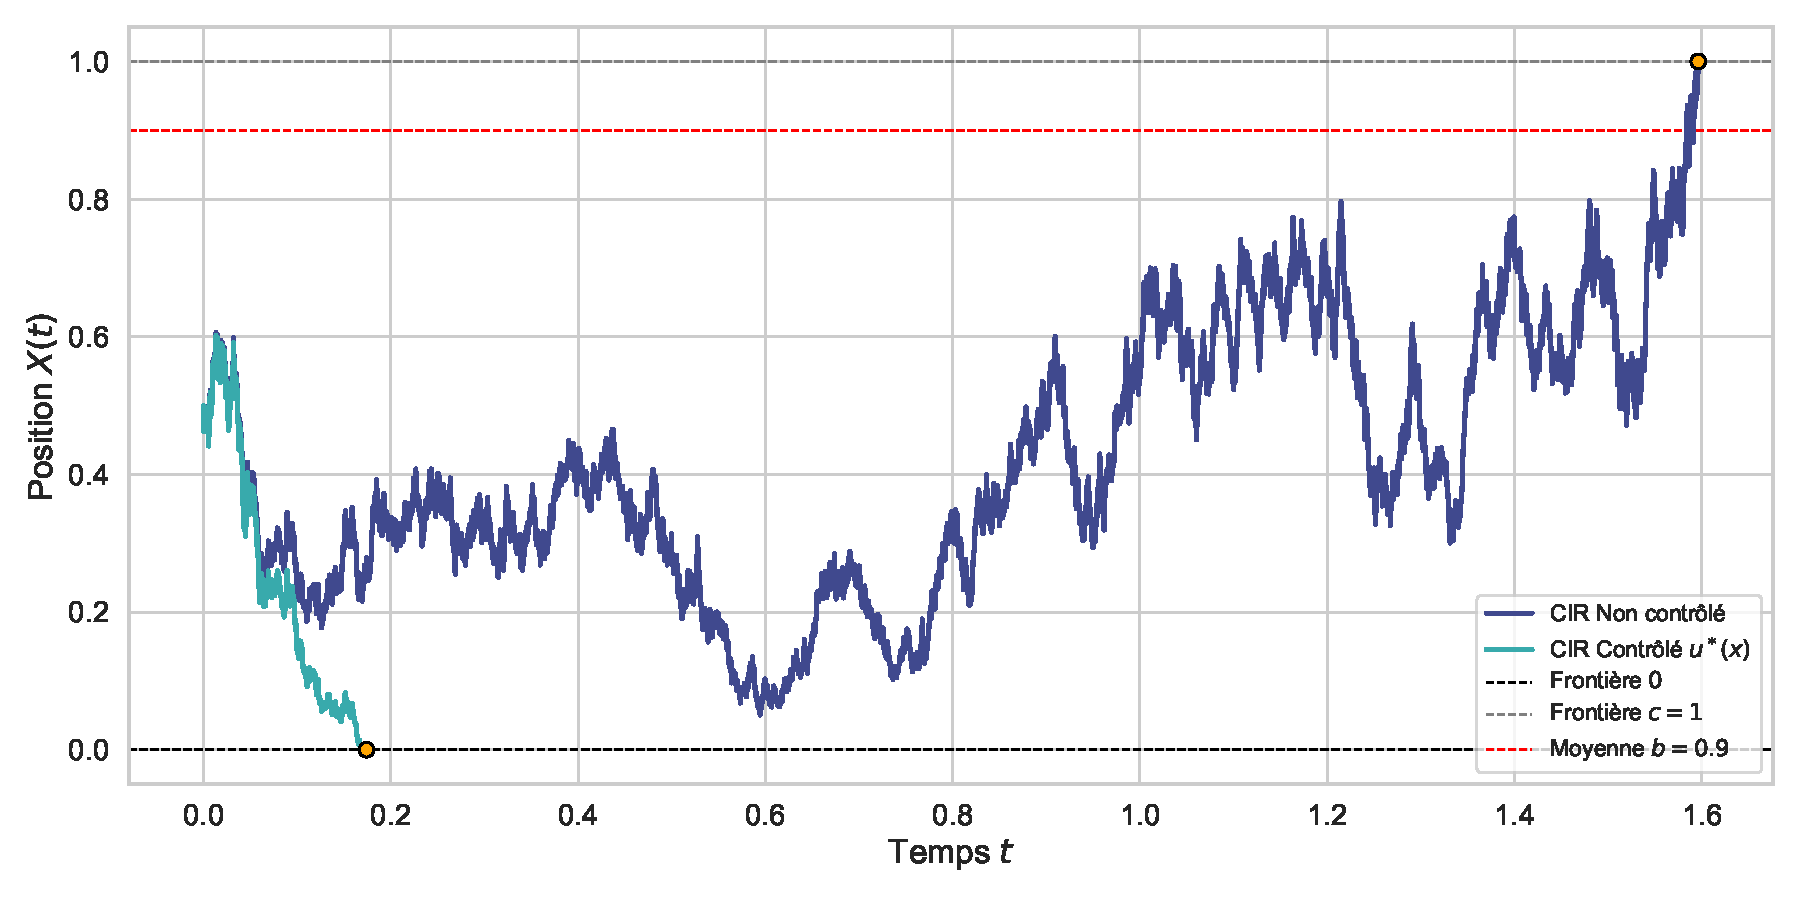
\includegraphics[width=0.9\linewidth]{img/validation/P2/p2_control_simulation.pdf}
    \caption{P2 \textemdash~Visualisation de l'effet de la commande optimale}\label{fig:Simulation2}
\end{figure}\FloatBarrier\subsection{P3 \textemdash~Résolution}\label{p3}
Soit le problème suivant:
\begin{itemize}
    \item $r(x) = x^2$: coût immédiat quadratique en $x$, indépendant du contrôle;
    \item $b(x) = x$: coût du contrôle linéaire égal à $x$;
    \item $q(x) \equiv 1$: poids pénalisant l'intensité du contrôle constant.
\end{itemize}
La condition (\ref{condition}) n'étant pas satisfaite, ce problème ne permet pas une linéarisation facile. Il faut donc le résoudre d'une autre manière. En éliminant le retour à la moyenne ($a=0$) et en posant $\sigma=1$, l'équation (\ref{control_equation}) se réduit à:
\begin{equation}\label{reduced_control_equation}
    x^2-\frac{x^2}{2}{F'(x)}^2+\frac{1}{2}xF''(x)=0
\end{equation}
Le logiciel de calcul symbolique \textit{Maple} donne comme solution pour $F(0)=0$ (avec $C_1$ une constante à déterminer):
\[
    F(x)=\int_0^x-\sqrt{2}\tanh\left(\frac{\sqrt{2}z^2}{2}+C_1\sqrt{2}\right)dz
\]
En posant $c=1$, la valeur de $C_1$ qui satisfait $F(c)=F(1)=0$ est $C_1\simeq -0.1652$. Donc, la forme finale de la fonction valeur est obtenue:
\begin{equation}\label{sol_control_3}
    F(x)\simeq \int_0^x-\sqrt{2}\tanh\left(\frac{\sqrt{2}z^2}{2}-0.1652\sqrt{2}\right)dz
\end{equation}
La commande optimale est donc:
\begin{equation}\label{optimal_control_3}
    u^*(x)\simeq x\sqrt{2}\tanh\left(\frac{\sqrt{2}x^2}{2}-0.1652\sqrt{2}\right)
\end{equation}
\subsection{P3 \textemdash~Visualisation}
La fonction valeur (\ref{sol_control_3}) ainsi que la commande optimale (\ref{optimal_control_3}) sont tracés.
\begin{figure}[htb]
    \centering
    \begin{subfigure}{0.45\linewidth}
        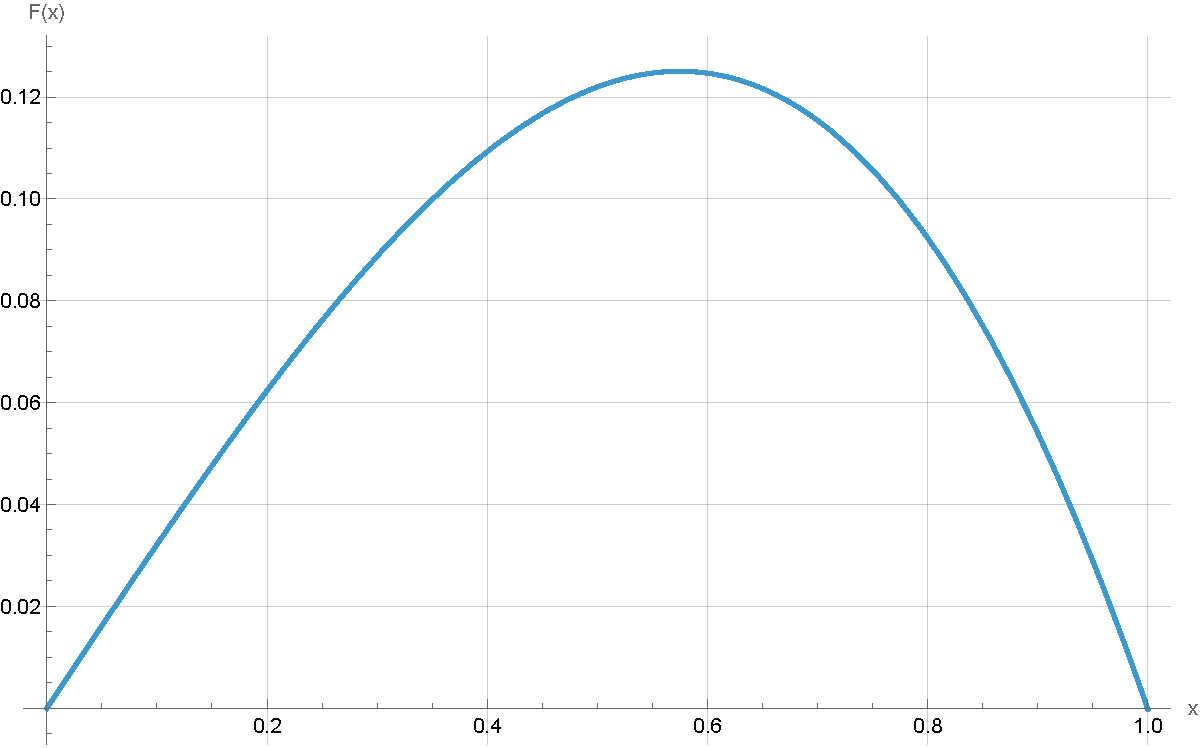
\includegraphics[width=\linewidth]{img/validation/P3/p3_value.pdf}
        \caption{P3 \textemdash~Fonction Valeur $F(x)$}\label{fig:ValueVisualisation3}
    \end{subfigure}
    \hfill
    \begin{subfigure}{0.45\linewidth}
        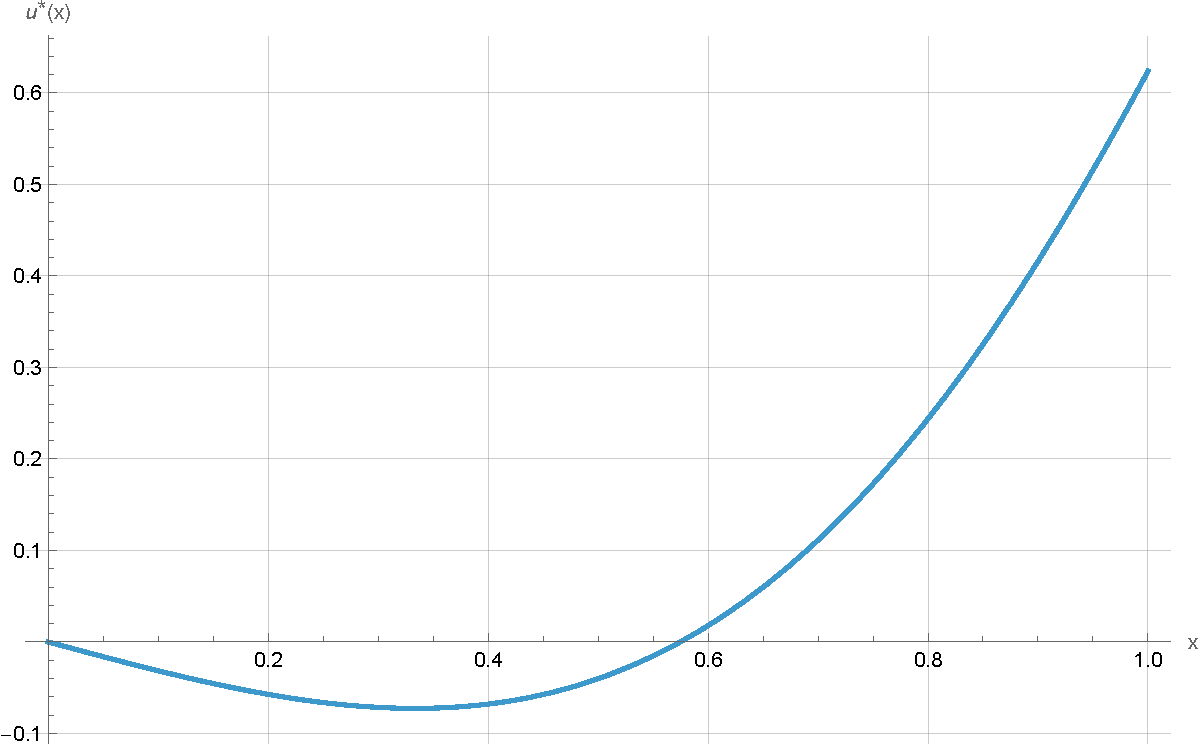
\includegraphics[width=\linewidth]{img/validation/P3/p3_control.pdf}
        \caption{P3 \textemdash~Contrôle Optimal $u^*(x)$}\label{fig:ControlVisualisation3}
    \end{subfigure}
    \caption{P3 \textemdash~Visualisation de la fonction valeur et du contrôle optimal}\label{fig:ValueControlComparison3}
\end{figure}
\FloatBarrier Enfin, une simulation est aussi effectuée. 
\begin{figure}[htb]
    \centering
    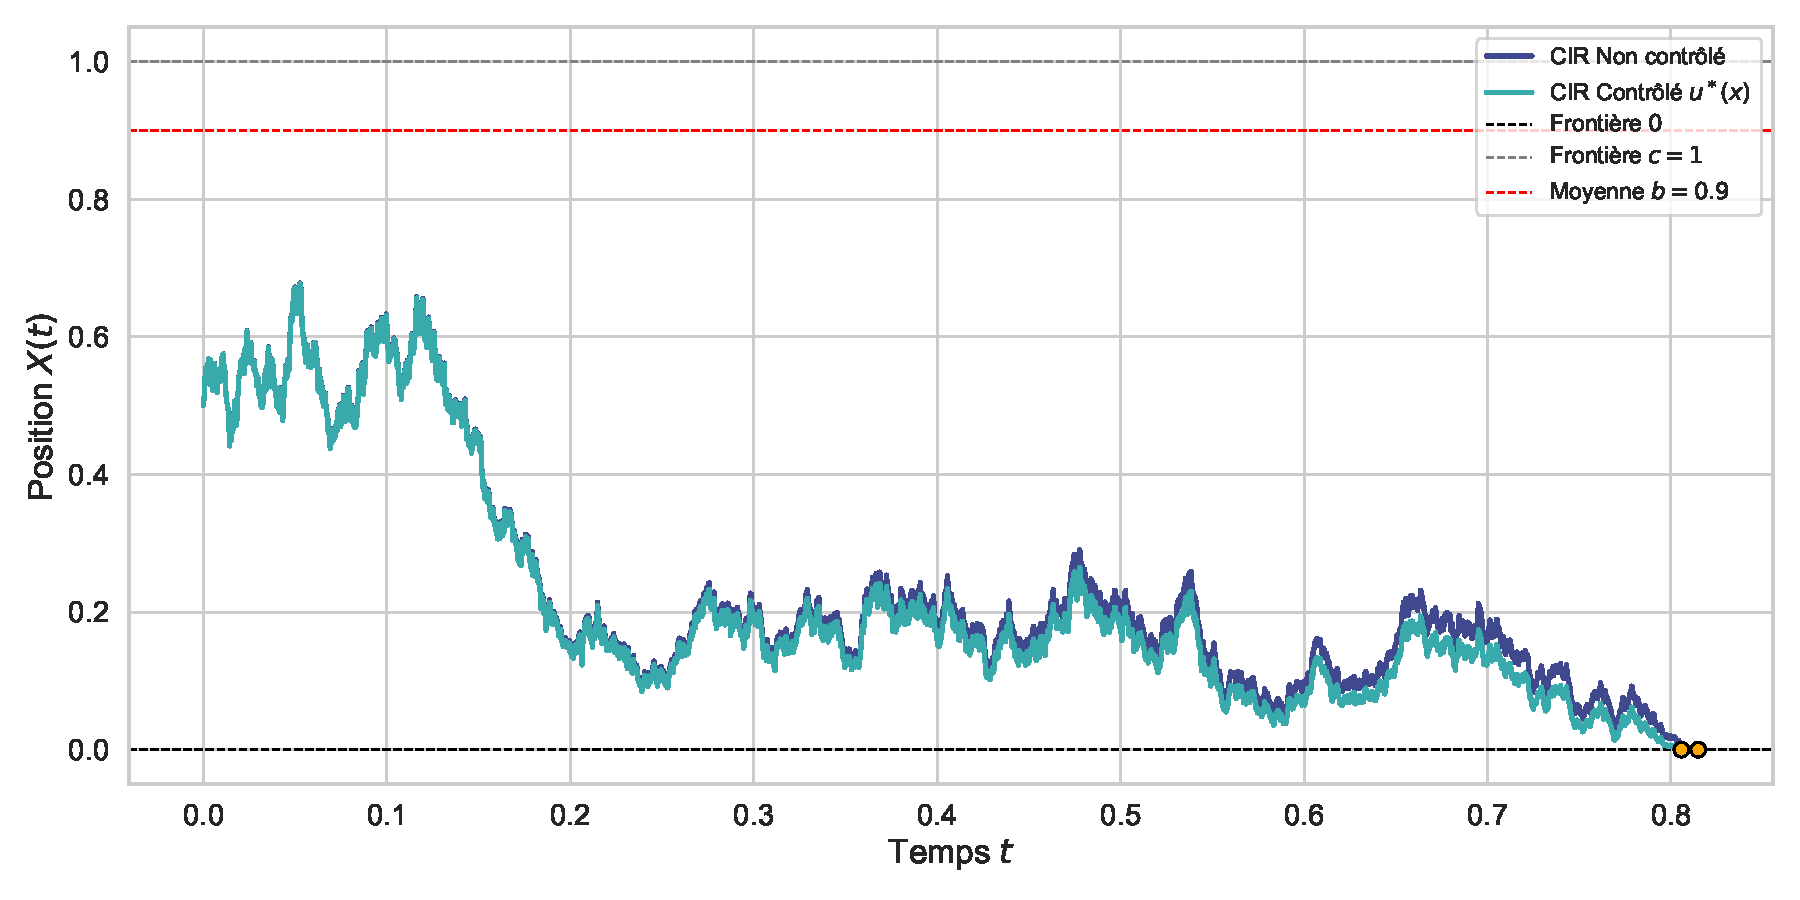
\includegraphics[width=0.9\linewidth]{img/validation/P3/p3_control_simulation.pdf}
    \caption{P3 \textemdash~Visualisation de l'effet de la commande optimale}\label{fig:Simulation3}
\end{figure}\FloatBarrier\section{Validation}
Il est important de souligner que, dans les trois problèmes étudiés et pour les différentes valeurs des paramètres considérés:
\begin{itemize}
    \item Les conditions aux limites $F(0)=F(c)=0$ sont toujours respectées;
    \item La fonction valeur est toujours positive, le coût encouru étant nécessairement positif;
    \item Le contrôle optimal est négatif lorsque \( x \to 0^+ \), l'optimiseur cherchant à diriger rapidement le processus vers la frontière inférieure, plus proche. Inversement, pour \( x \to c^-\), le contrôle devient positif afin d'accélérer l'atteinte de la frontière supérieure;
    \begin{sloppypar}\item Une augmentation du coût immédiat $\rho$, induisant une hausse du coût encouru (\ref{fig:RhoValueVisualisation1},~\ref{fig:RhoValueVisualisation2}), entraîne un renforcement du contrôle optimal ($|u^*(x)|$ augmente dans~\ref{fig:RhoControlVisualisation1} et~\ref{fig:RhoControlVisualisation2}), traduisant ainsi une volonté accrue de quitter l'intervalle aussi rapidement que possible;\end{sloppypar}
    \item Une hausse du coût du contrôle $\beta$ incite à intensifier le contrôle optimal (\ref{fig:BetaControlVisualisation1},~\ref{fig:BetaControlVisualisation2}) afin de quitter l'intervalle plus rapidement. Cette stratégie réduit la durée d'exposition au coût instantané, ce qui compense partiellement le surcoût du contrôle et diminue le coût total encouru $F(x)$ (\ref{fig:BetaValueVisualisation1},~\ref{fig:BetaValueVisualisation2});
    \item Une augmentation du poids pénalisant le contrôle $\kappa$, induisant une hausse du coût encouru (\ref{fig:KappaValueVisualisation1},~\ref{fig:KappaValueVisualisation2}), entraîne une relaxation du contrôle optimal (\ref{fig:KappaControlVisualisation1},~\ref{fig:KappaControlVisualisation2}). En effet, plus le poids du contrôle est élevé, moins il est intéressant d'appliquer un contrôle fort;
    \item Les simulations (\ref{fig:Simulation1},~\ref{fig:Simulation2},~\ref{fig:Simulation3}) mettent en évidence l'effet du contrôle optimal, qui accélère la sortie du processus par rapport au cas non contrôlé. Pour valider cette observation, 1000 trajectoires sont simulées pour chaque problème, et la durée moyenne jusqu'à la sortie est comparée. Un facteur d'accélération est ensuite estimé (voir annexe~\ref{control_simulations} pour les détails du calcul):
    \begin{table}[htb]
        \centering
        \caption{Accélérations moyennes du temps de sortie}\label{tab:acceleration_results}
        \renewcommand{\arraystretch}{1.1}
        \begin{tabular}{||c|c||}
        \hline
        Problème & Accélération Moyenne \\\hline\hline
        P1 & 2.660552 \\
        P2 & 2.690582 \\
        P3 & 1.065163 \\\hline
        \end{tabular}
    \end{table}
\end{itemize}\FloatBarrier Ainsi, les expressions obtenues pour la fonction valeur $F(x)$ et le contrôle optimal $u^*(x)$ sont validées.

Ces observations générales fournissent un cadre d'interprétation cohérent pour les stratégies optimales. Ces dernières sont détaillées dans la partie qui suit.
\section{Politiques Optimales}
À partir des simulations réalisées, de l'analyse des profils des commandes optimales \( u^*(x) \) illustrés dans les figures~\ref{fig:ControlVisualisation1},~\ref{fig:ControlVisualisation2} et~\ref{fig:ControlVisualisation3}, ainsi que de leur mise en relation avec les structures de coûts propres à chaque configuration, il est possible de caractériser précisément les différentes stratégies de contrôle optimales associées à chacun des problèmes étudiés:
\begin{itemize}
    \item \textbf{Stratégie P1}: La politique optimale en configuration P1 adopte une structure à seuil, avec un point critique situé autour de \(x^* \approx 0.33\). Pour \(x < x^*\), le contrôle diverge rapidement vers \(-\infty\), tirant agressivement le processus vers la borne inférieure. Ce comportement traduit une exploitation stratégique de la structure des coûts \(b(x) = q(x) = x\), qui tendent eux aussi vers zéro, rendant le contrôle intensif peu pénalisant dans cette région. Inversement, pour \(x > x^*\), le contrôle devient positif mais reste modéré, poussant le processus vers la borne supérieure de l'intervalle jusqu'à \(u(1)\approx1.4\).

    L'asymétrie du seuil observée dans cette politique s'explique par la nature du coût d'état constant \(r(x)\equiv1\) ainsi que deux mécanismes complémentaires. Premièrement, la dynamique du processus \acs{CIR} possède un terme de retour à la moyenne dirigé vers \(b\) (fixé ici à 0.9). Ainsi, dès que le processus est situé en dessous de cette valeur, il bénéficie naturellement d'une poussée ascendante, ce qui rend avantageux de renforcer cette tendance au-delà du seuil \(x^*\) par un contrôle positif. Deuxièmement, la diffusion du processus étant proportionnelle à \(\sqrt{X(t)}\), les perturbations aléatoires sont fortement atténuées près de zéro. Il est donc inefficace de chercher à atteindre la borne inférieure depuis une position trop éloignée, et le contrôle n'est justifié dans cette direction que pour des valeurs suffisamment petites de \(x\) (en-dessous du seuil $x^*$). Ce comportement est corroboré par une analyse empirique: sur 1000 trajectoires simulées, le processus s'échappe par la borne supérieure dans 67\,\% des cas (voir~\ref{tab:simulation_exit_frequency});
    \item \textbf{Stratégie P2}: Ici, la politique optimale présente également une structure à seuil, avec un point de bascule situé à \( x^* \approx 0.56 \). Au-delà de ce seuil, la commande coïncide avec celle observée en P1, adoptant une forme croissante et positive jusqu'à \(u(1)\approx1.4\). En revanche, pour \( x < x^* \), le contrôle décroît rapidement et atteint un minimum marqué autour de \( u(0.07) \approx -2.2 \). Ce comportement reflète une stratégie visant à tirer activement le processus vers la frontière inférieure, profitant de la faible pénalisation induite par la structure des coûts \( b(x) = \sqrt{x} \) et \( r(x) = q(x) = x \), qui deviennent négligeables à proximité de zéro.
    
    Un aspect notable est que le contrôle s'annule en \( x = 0 \). L'optimiseur privilégie alors une stratégie en deux temps: amener le processus vers une zone proche de \( x = 0.07 \), où un contrôle négatif fort est encore efficace et peu coûteux, puis relâcher l'effort pour laisser la dynamique intrinsèque du processus conduire la sortie par la borne inférieure. Une fréquence expérimentale de sortie par la borne inférieure de 66.7\,\% vient valider ce comportement (\ref{tab:simulation_exit_frequency});
    \item \textbf{Stratégie P3}: La politique optimale correspond à une stratégie d'évasion passive. Bien qu'un seuil \(x^*\) subsiste, marquant l'inversion du signe de la commande, l'amplitude de \(u(x)\) demeure globalement faible. En effet, avec un poids pénalisant l'intensité du contrôle constant \(q(x) \equiv 1\), l'optimiseur n'est pas particulièrement incité à appliquer une commande intensive. Celui-ci n'intervient donc que de manière ponctuelle et uniquement lorsque cela s'avère nécessaire, sans chercher à forcer activement la dynamique du processus. Ce comportement est confirmé par le faible facteur d'accélération observé, estimé à 1.06 (voir~\ref{tab:acceleration_results}), ainsi qu'une fréquence de sortie pour chaque frontière presque identique à celle du processus non-contrôlé (\ref{tab:simulation_exit_frequency}), indiquant une quasi-absence de différence entre les trajectoires contrôlées et non contrôlées.
\end{itemize}
